\documentclass{article}
\usepackage{graphicx}
\usepackage{subfig}
\usepackage{color}
\usepackage{appendix}




\sloppy
\definecolor{lightgray}{gray}{0.5}
\oddsidemargin 0.2in
\evensidemargin 0.2in
\textwidth 6.0in
\textheight 8.0in
\topmargin 0.2in

\begin{document}
\title{\textbf{CSCI5552: Sensing and Estimation in Robotics \\ SLAM Project} \\ Interim Report}
\author{Manish Prahladka\\
				Anoop Cherian\\
				Ravishankar Sivalingam}

\maketitle

\section{Introduction}

We design and implement the Simultaneous Localization and Mapping (SLAM) algorithm on the Pioneer3 series of robots available from ActiveMedia Robotics. Our goals are to:\\ \\
-- design and implement a feature extraction algorithm to extract environment features in an indoor environment\\
-- design and implement a localization scheme based on the extracted feature information \\
-- integrate the above two to develop a automatic navigation algorithm, while simultaneously constructing a localization map 

Right now we have pulled much of the code from last years Parallel Parking code. As of right now our robot can align itself to a wall, detect corner features and make turns. We are using a laser scanner range based algorithm to decide when to turn. This algorithm also gives the robot a sense of basic obstacle avoidance without additional code as it detects obstacles as features and tries to avoid them. The robot does not have a sense of its own width or position as much so it 'tries' to avoid the object but bumps into them. \\

***** add more info to current range finding algorithm

\section{Feature Extraction}

We are implementing the feature extraction algorithm using the SICK 200 laser scanners available with the Pioneer3 series of robots. The laser scans are processed using the ArLineFinder class available in the ARIA libraries. The algorithm tries to fit lines to the laser scan data and we determine point features (with respect to which we have to localize the robots), by finding the points of intersection of these lines. The feature extraction is working as of right now and much of the code was just pulled from last years parallel parking project.\\

***** add information on how we obtained the map

Here is the map we obtained:
\begin{figure}[htb] 
\centering
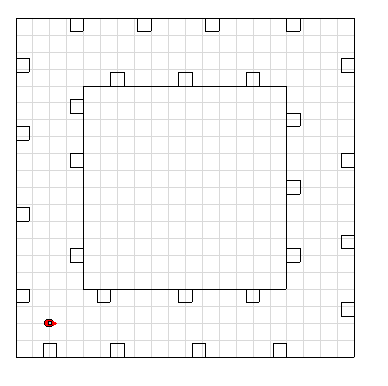
\includegraphics[width=0.5\textwidth]{map.png}
\caption {Map of the Corridor}
\end{figure}

\section{Filtering and localization}

Using the extracted features from algorithm, we implement a Extended Kalman Filter to combine the sensor readings with the robot's odometric pose estimates. We have implemented the propagate step of the Kalman Filter using some dummy data and incorporated the optimizations discussed in class in that code. We had to implement our own template based matrix class to implement this and we are adding to the class as we go. What needs to be done :\\ \\
--Implement the EKF update step\\
--Wrap the update and propagate steps in appropriate threads\\
--Make it compatible with our feature extraction algorithm\\
--Figure out thread timings and synchronization issues to make the system work as a whole.\\


\end{document}    

